%--------------------------------------------------------------------
% NENG 685 (intro to methods for neutral particle transport)

\documentclass[12pt]{article}
\usepackage[top=1in, bottom=1in, left=1in, right=1in]{geometry}

\usepackage{setspace}
\onehalfspacing

\usepackage{amssymb}
%% The amsthm package provides extended theorem environments
\usepackage{amsthm}
\usepackage{epsfig}
\usepackage{times}
\renewcommand{\ttdefault}{cmtt}
\usepackage{amsmath}
\usepackage{graphicx} % for graphics files
\usepackage{tabu}

% Draw figures yourself
\usepackage{tikz} 

% The float package HAS to load before hyperref
\usepackage{float} % for psuedocode formatting
\usepackage{xspace}

% from Denovo Methods Manual
\usepackage{mathrsfs}
\usepackage[mathcal]{euscript}
\usepackage{color}
\usepackage{array}

\usepackage[pdftex]{hyperref}
\usepackage[parfill]{parskip}

% math syntax
\newcommand{\nth}{n\ensuremath{^{\text{th}}} }
\newcommand{\ve}[1]{\ensuremath{\mathbf{#1}}}
\newcommand{\Macro}{\ensuremath{\Sigma}}
\newcommand{\rvec}{\ensuremath{\vec{r}}}
\newcommand{\vecr}{\ensuremath{\vec{r}}}
\newcommand{\omvec}{\ensuremath{\hat{\Omega}}}
\newcommand{\vOmega}{\ensuremath{\hat{\Omega}}}
\newcommand{\sigs}{\ensuremath{\Sigma_s(\rvec,E'\rightarrow E,\omvec'\rightarrow\omvec)}}
\newcommand{\el}{\ensuremath{\ell}}
\newcommand{\sigso}{\ensuremath{\Sigma_{s,0}}}
\newcommand{\sigsi}{\ensuremath{\Sigma_{s,1}}}
%---------------------------------------------------------------------------
%---------------------------------------------------------------------------
\begin{document}
\begin{center}
{\bf NENG 685, Fall 17 \\
Introduction to Monte- Carlo\\
October 30, 2017}
\end{center}

\section*{Learning Objectives}

After the class and assignments related to this material, you should be able to 
\begin{enumerate}
  \item Track particles through a geometry
  \item Use mean free paths to sample the distance to the next physics event
  \item Sample the physics event that occurred
  \item Translate interations into a score 
\end{enumerate}

\section*{Tracking Particles}

Recall from lesson 8, that a basic MC algorithm can be specified as \autoref{fig: mc_algo}.

\begin{figure}[h!]
\begin{center}
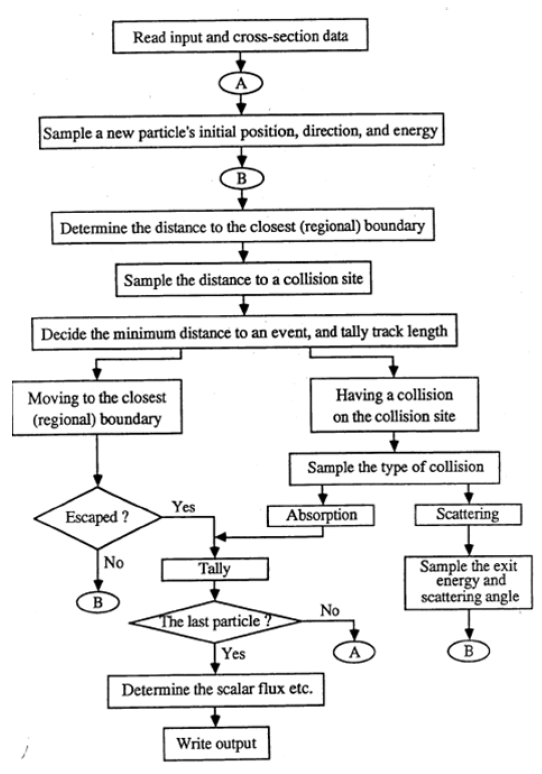
\includegraphics[scale=0.80]{../figs/mcAlgo.png}
\caption{Basic MC algorithm for radiation transport}
\label{fig: mc_algo}
\end{center}
\end{figure}

After we have read in the data and sampled our starting location, we have a neutral particle that is

\begin{itemize}
  \item At point ($x_p$, $y_p$, $z_p$)
  \item Moving in direction ($u$, $v$, $w$)
  \item With energy E.
\end{itemize}

The next possible events are a collision (interaction) - shown in \autoref{fig: collision}

\begin{figure}[h!]
\begin{center}
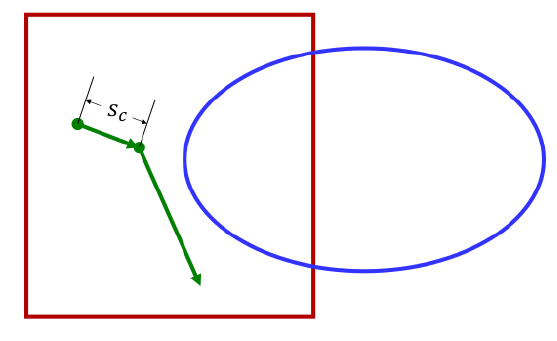
\includegraphics[scale=0.80]{../figs/collision.png}
\caption{Collision Event}
\label{fig: collision}
\end{center}
\end{figure}

or a surface crossing - shown in \autoref{fig: surface-crossing}

\begin{figure}[h!]
\begin{center}
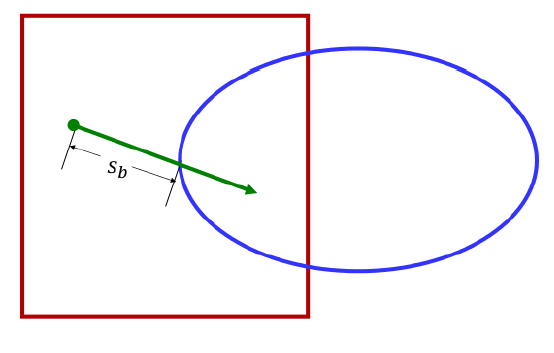
\includegraphics[scale=0.80]{../figs/surface-crossing.png}
\caption{Surface Crossing Event}
\label{fig: surface-crossing}
\end{center}
\end{figure}

Collisions are probabilistic (which is why MC works so well!), and can be defined as the probability of occurring at a distance, $s$ from the start according to

\begin{align*}
    p_c(s)ds &= \Sigma_t(s) e^{-\Sigma_t(s) s} ds \\
    P_c(s) &= \int_0^s \Sigma_t(s) e^{-\Sigma_t(s) s'}ds' = -e^{-\Sigma_t(s) s'} |_0^s = 1 - e^{-\Sigma_t(s) s}
\end{align*}

The total cross section, $\Sigma_t(s)$ is piece-wise constant, but changes with material.
To overcome this, we can do a variable transformation and measure distances in units of \textit{mean free path (MFP)}:

\begin{align*}
    n &= \Sigma_t(s)s \\
    dn &= \Sigma_t(s)ds.
\end{align*}

We can then define the PDF and CDF as 

 \begin{align*}
    p_c(n)dn &= e^{-n} dn\\
    P_c(n) &= \int_0^n e^{-n'}dn' = -e^{-n'} |_0^n = 1 - e^{-n}.
  \end{align*}

This is now independent of material, and we can sample the number of MFPs until next collision, $n_c$ :

\begin{itemize}
  \item $g(n_c) dn_c = e^{-n_c} dn_c$ 
  \vspace{.5em}
  \item $G(n_c) dn_c = 1 - e^{-n_c}$ 
  \vspace{.5em}
  \item Directly invert to get: $\boxed{n_c = - \ln(1 - \xi)}$ \\
   \hspace*{1.5em} [note $(1-\xi)$ is equivalent to $\xi$]
  \vspace{.5em}
  \item In the absence of material boundaries ($\Sigma_t \neq f(s)$), the distance to a collision, $s_c$, is
  \[s_c = \frac{n_c}{\Sigma_t}\]
\end{itemize}

However, we usually have more than one material (hence the need to go to MFP sampling in the first place).
Given that our particles move in predicable straight lines, the distance to the next boundary is deterministic and can be calculated using Algebra to determine the distance between a point and the next surface, $s_b$.  
We can then convert this to units of mean free path for the current cell's material:

\begin{equation}
  n_b = s_b \sigma_t
\end{equation}

In MC codes, the geometry is typically represented using 

\begin{itemize}
  \item Combinatorial Surfaces
  \begin{itemize}
    \item Define surfaces
    \item Boolean operations combine surfaces to create cells
  \end{itemize}
  \vspace*{1 em}
  \item Combinatorial Solids
  \begin{itemize}
    \item Choose solid objects
    \item Boolean operations combine objects to create regions
  \end{itemize}
  \vspace*{1 em}
  \item B-Rep (Vertex-Edge)
  \begin{itemize}
    \item Each object is a single set of vertices and edges connecting them
  \end{itemize}
\end{itemize}

We will not define how to calculate $s_b$ for each situation.

Ok, we have sampled the distance to the next collision, so what's next?
If we refer to \autoref{fig: mc_algo}, we see we are at a decision point.
The options are:

\underline{$n_b > n_c$}:
\begin{itemize}
  \item Boundary is further away than collision
  \item Collision occurs
\end{itemize}
  \vspace*{0.5 em}

\begin{itemize}
  \item Using physics models and/or cross-sections
  \begin{itemize}
    \item Sample target nuclide
    \item Sample reaction type
    \item Sample new direction 
    \item Sample new energy 
    \item Sample exiting particles 
  \end{itemize}
  \item Some of these may depend on one another
  \vspace*{0.5 em}
  \item Repeat
  \begin{itemize}
    \item Sample new $n_c$ following collision
    \item Calculate new $n_b$ in new direction
  \end{itemize}
\end{itemize}  
  
\underline{$n_b < n_c$}:
\begin{itemize}
  \item Boundary is closer than collision
  \item Boundary crossing occurs
\end{itemize}

\begin{itemize}
  \item Move particle along ray
  \begin{itemize}
    \item Update $n_c = n_c - n_b$
  \end{itemize}
  \item \textbf{DO NOT SAMPLE} for new $n_c$
  \vspace*{1 em}
  \item Calculate new $n_b$ in new cell
  \begin{itemize}
    \item New set of boundaries
    \item New value of $\Sigma_t$
  \end{itemize}
\end{itemize}

If we have a collision, we then need to determine which nuclide was hit (if there are multiple, which there often are) and which reaction occurred.
The steps involved are:

\begin{itemize}
  \item Sample \textbf{target nuclide} for a mixture with $J$ nuclides
    \[\Sigma_t = \sum_{j=1}^J N_j \sigma_{t,j}\]
  \item \textit{Discrete PDF} to determine which nuclide is hit
    \[p_j = \frac{\Sigma_{t,j}}{\Sigma_t}\]
  \item Sample \textbf{reaction type} for an nuclide with R types of reactions
     \[\Sigma_{t,j} = \sum_{x=1}^R \Sigma_{x,j}\]
  \item \textit{Discrete PDF} to determine which reaction occurs
    \[p_x = \frac{\Sigma_{x,j}}{\Sigma_{t,j}}\]
\end{itemize}

\subsection*{Reaction Outcomes}

After the collision, there are a couple of possible outcomes for our neutral particle:

\begin{itemize}
    \item Particle maybe absorbed
    \item Particle may continue its history in a \textit{different direction} and/or with a \textit{different energy}
\end{itemize}

If the particle is to continue, we need to sample the new energy-angle distribution.  
Each is tabulated in different formats:

\begin{itemize}
  \item Scattering laws have analytic forms with parameters in data tables\\
        (Direct inversion or rejection sampling)
  \item Tabulated data that describes a piecewise analytic interpolation\\
      (Hybrid sampling; we skipped this)
\end{itemize}

\subsection*{Scattering Angle}

Scattering angles are defined relative to the original direction (considered as the z-axis)

\begin{itemize}
    \item Polar angle, $\phi$, determined by sampling from data
\vspace*{0.5em}
    \item Azimuthal angle, $\theta$, determined by sampling isotropically
    \vspace*{0.5em}
    \item The new direction is $\bigl(\sin(\theta) \cos(\phi), \sin(\theta) \sin(\phi), \cos(\phi)\bigr)$ \[= \bigl(\sqrt{1 - \mu^2} \cos(\theta),  \sqrt{1 - \mu^2} \sin(\theta), \mu \bigr)\]
\end{itemize}

This is shown graphically in \autoref{fig: scattering-angle-2}.

\begin{figure}[h!]
\begin{center}
  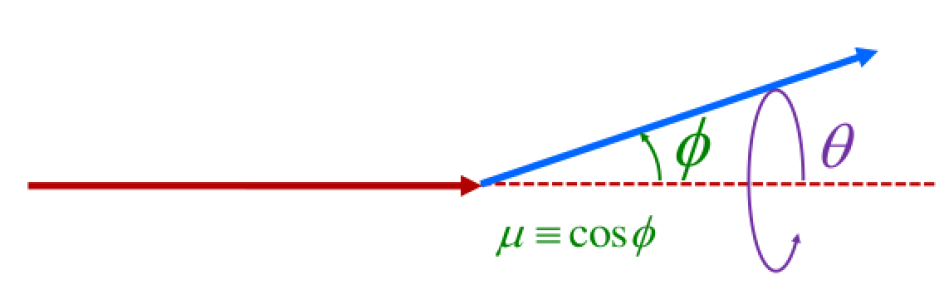
\includegraphics[height=1in,clip]{../figs/scattering-angle-2.png}
  \caption{Scattering angle diagram.}
  \label{fig: scattering-angle-2}
\end{center}
\end{figure}


\section*{Scoring}

Now that we know what happens at the collision site, we need to formalize how we score (tally) the results for radiation transport.

We have shown how to generate a collection of histories.\\
Each history, $i$, is just a series of interaction sites.\\
\textit{Estimators} convert each history into a score, $x_i$. \\
Each history has a different score (in general).\\
A \textit{tally} accumulates a set of scores, $\{x_i\}$, to form a probability density function.

Usually we're interested in the \textit{expected value} of the underlying PDF. \\
Tallies are \textit{normalized} to the number of source particles. Thus
\[
E(x) = \frac{1}{N} \sum_{i=1}^N x_i
\]
where $N$ is the number of MC particles in the simulation source.\\
The absolute physical quantities require multiplication by the physical source strength (check for a given Monte Carlo code to ensure this is the way it works). 

Typically, we can choose to subdivide phase space into domains or bins (energy bins for spectra, cosine bins for angular distributions, etc.) for the tallied response.

We have three main types of estimators for radiation transport:
\begin{enumerate}
\item point estimators: surface crossings (current tally, surface flux tally) and collisions (eigenvalue tally)
\item track length estimator: path length through a cell (volume flux tally)
\item energy balance estimator: energy loss in cell (pulse height tally)
\end{enumerate}
%
We can now develop the estimator scores with a weight value that scales its contribution to the tally.
For now the weight will always be $1$, so you can functionally ignore it. 
However, these weights will become important when considering variance reduction techniques (only briefly described in this class).

For a surface or current tally, we count particle crossing a surface:
\[
x_i = \sum_j w_{ij} \quad \text{summing over each crossing }j\text{ of history }i
\]
The current [particles] is
\[
\int_A dA \int_t dt \int_{\vOmega} d\vOmega \int_E dE\: \hat{n} \cdot \vec{J}(\rvec, E, t) \approx \frac{1}{N} \sum_{i}^N x_i = \frac{1}{N} \sum_{i}\sum_{j} w_{ij}=\frac{W}{N}
\]
And the surface energy current [MeV] is
\[
\int_A dA \int_t dt  \int_{\vOmega} d\vOmega \int_E dE\: E\hat{n} \cdot \vec{J}(\rvec, E) \approx \frac{1}{N} \sum_{i}\sum_{j} E_{ij}w_{ij} = \frac{E_T\:W}{N}
\]

To get the flux/fluence in a volume
\[
\bar{\phi_V} = \frac{1}{V}\int_V dV \int_t dt \int_E dE\: \phi(\rvec, E,t) =  \frac{1}{V}\int_V dV \int_s ds \int_E dE\: N(\rvec, E,t)
\]
where we noted that $\phi \equiv vN$ and then $vdt = ds$.\\
We can now see that we can use either a collision or a track length estimator for flux.\\
Collision (score happens at collision of particle $i$):
\[
\bar{\phi_V} \approx \frac{1}{V}\frac{1}{N} \sum_{i} x_i = \frac{1}{V}\frac{1}{N} \sum_{i} w_i = \frac{W}{V \: N}
\]
Track length ($N(\rvec, E,t)ds$ is density of track lengths, $T_l$):
\[
\bar{\phi_V} \approx \frac{1}{V}\frac{1}{N} \sum_{i}\sum_{j} w_{ij}T_{l,ij} = \frac{W \: T_l}{V \: N}
\]

Surface flux can also be obtained with track length tallies by accounting for angle of crossing, $\theta$ and $\mu_{ij} = \cos(\theta_{ij})$. Assume we're thinking of a volume cell that becomes infinitely thin with thickness $\delta$. 
\begin{align*}
T_{l,ij} &= \frac{\delta}{|\cos(\theta_{ij})|}\\
\bar{\phi_A} &\approx \frac{1}{V}\frac{1}{N} \sum_{i=1}\sum_{i=j} w_{ij}\frac{\delta}{|\mu_{ij}|} = \frac{1}{A \delta}\frac{1}{N} \delta \sum_{i=1}\sum_{i=j} \frac{w_{ij}}{|\mu_{ij}|} = \frac{W}{|\mu | \: A \: N}
\end{align*}
%
And so on for other items of interest.  
Chapter 2 of the MCNP manual has a great description of common tallies for MC methods.

%-------------------------------------------------------
%-------------------------------------------------------\\
\section*{Statistics}
The ``true" mean value, $\mu$, of any PDF is the expected value, $E(x)$
\[
\mu = E(x) = \int x f(x) dx
\]
Because we can't usually do this, we use random samples and estimate the true mean from the ``sample" mean, $\bar{x}$
\[
\bar{x} = \frac{1}{N}\sum_{i=1}^N x_i \qquad \lim_{N \to \infty} \bar{x} \rightarrow \mu\:.
\]
The variance of a PDF is the measure of spread in that PDF
\begin{align*}
\sigma^2 &= E[(x - \mu)^2] = \int (x - \mu)^2 f(x) dx \\
&= \int x^2 f(x) dx - 2 \mu \int x f(x) dx + \mu^2 \int f(x) dx\\
&= E(x^2) - \mu^2
\end{align*}
%
However, we don't know the PDF so we use the samples to get the sample variances
\begin{align*}
S_x^2 &= \frac{1}{N-1}\sum_{i=1}^N (x_i - \bar{x})^2 \\
&= \frac{1}{N-1} \biggl[\sum_{i=1}^N x_i^2 - 2 \bar{x}\sum_{i=1}^N x_i + \bar{x}^2 \sum_{i=1}^N 1 \biggr] 
\end{align*}

The \underline{Central Limit Theorem} states that
For $N$ \textit{independent} random variables, $x_i$, sampled from \textit{identical distributions}, their mean follows a Normal (Gaussian) distribution.\\
We can use this information to define \textit{confidence intervals}
\begin{align*}
\bar{x} - S_{\bar{x}} &< E(x) < \bar{x} + S_{\bar{x}} \quad \text{about 68\% of the time}\\
\bar{x} - 2S_{\bar{x}} &< E(x) < \bar{x} + 2S_{\bar{x}} \quad \text{about 95\% of the time}
\end{align*}

The \textbf{standard deviation} of the mean is a measure of the error in the result
\begin{align*}
S_{\bar{x}}^2 &= E[(\bar{x} - \mu)^2] = E\biggl[ \biggl(\frac{1}{N}\sum_{i=1}^N x_i - \mu\biggr)^2\biggr] = E\biggl[ \biggl(\frac{1}{N^2}\sum_{i=1}^N (x_i - \mu)\biggr)^2\biggr]\\
%
&=\frac{1}{N^2} E\biggl[ \sum_{i=1}^N (x_i - \mu) \sum_{j=1}^N (x_j - \mu)\biggr] = \frac{1}{N^2} E\biggl[ \sum_{i=1}^N \sum_{j=1}^N (x_i - \mu)  (x_j - \mu)\biggr]\\
%
&= \frac{1}{N^2} \sum_{i=1}^N \sum_{j=1}^N E\bigl[  (x_i - \mu)  (x_j - \mu)\bigr] = \frac{1}{N^2} \sum_{i=1}^N \sum_{j=1}^N S^2_x \delta_{ij} = \frac{1}{N^2} \sum_{i=1}^N S_x^2 \\
%
&= \frac{N S_x^2}{N^2} = \boxed{\frac{S_x^2}{N}}
\end{align*}
The error in the results decreases with the square root of increasing the number of histories.
%
\begin{figure}[h!]
\begin{center}
  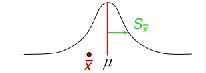
\includegraphics[height=1 in,clip]{../figs/gaussian.jpg}
\end{center}
  %\caption{Monte Carlo neutral particle transport algorithm}
  \label{fig:gaussian}
\end{figure}

\textbf{Relative Error} is 
\[
R = \frac{S_{\bar{x}}}{\bar{x}} = \sqrt{\frac{\sum_{i=1}^N x_i^2}{\bigl(\sum_{i=1}^N x_i\bigr)^2} - \frac{1}{N}} 
\]
If $x_i$ are equal and non-zero, R=0.\\
Thus, we can reduce the error by reducing the spread in $x_i$.

\subsection*{Accuracy vs.\ Precision}
The distinction between accuracy and precision can be seen in Fig.~\ref{fig:accuracy}.\\
%
\begin{figure}[h!]
\begin{center}
  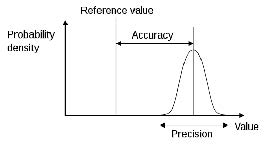
\includegraphics[height=2 in,clip]{../figs/accuracy-and-precision.jpg}
\end{center}
  \label{fig:accuracy}
\end{figure}
%
\textit{Accuracy} is the degree of closeness of measurements of a quantity to that quantity's true value.\\
The \textit{precision} of a measurement system, related to reproducibility and repeatability, is the degree to which repeated measurements under unchanged conditions show the same results.
% https://en.wikipedia.org/wiki/Accuracy_and_precision

Accuracy can be affected by systematic errors in simulation: physical and mathematical models; errors in geometry or source model; incorrect code use by user.\\
Usually unknown.

Conversely, precision can usually be improved: run more histories; use variance reduction; adjust your measurement (fewer scoring bins).

\vspace*{1 em}
%-------------------------------------------------------
%-------------------------------------------------------
\section*{Variance Reduction}
What we have talked about so far is \textit{Analog} Monte Carlo:
\begin{itemize}
    \item Natural laws are \textbf{preserved}
    \item The game is the ``analog" of the physical problem of interest (the history of each particle is simulated exactly)
    \item No alteration of PDFs
    \item At collision, particle is killed if absorption
    \item Particle is born with weight 1
    \item weight unchanged throughout history
    \item Score when tallying events is 1
\end{itemize}
%
We often, instead, want to do \textit{Non-Analog} Monte Carlo:
\begin{itemize}
    \item To reduce computation time, the strict analog simulation of particles is abandoned
    \item Variance Reduction techniques: Absorption suppression, Russian Roulette (history termination), Splitting (history propagation), Forced collisions, Source biasing, Hybrid methods
    \item Alter PDFs to favor events of interest
    \item Particle can have different birth weight
    \item Weight is altered if biased PDF is used
    \item Particle survives ``absorption" and weight is changed
    \item Splitting and RR can change weight
    \item Score current weight when tallying
\end{itemize}
%
We'll talk about implicit capture (a.k.a.\ survival biasing), roulette, splitting, and weight window maps. 

The first thing to think about is how to measure success. How do we know if a calculation is ``better"?\\
We use the figure of merit
\[
FOM =\frac{1}{R^2 t}\:,
\]
where $R$ is the relative error and $t$ is the particle tracking time.\\
What we really want is to reduce both of these. \\
Why are they related to one another this way? Recall that $S_{\bar{x}} \propto \sqrt{\frac{1}{N}}$.\\
It's clear that without variance reduction techniques to reduce error by a factor of two you need to increase particle count (and hence time) by a factor of four.\\
FOM measures if we're really winning.

\textit{The idea of VR is to track particles that will contribute meaningfully to the desired results and to avoid tracking those that will not while maintaining a fair game.}

The implementation of VR techniques is beyond the scope of this class, but simple methods will be described for MCNP.

\end{document}
